\section{Step 6 --- Caption Token Representation and Input Conditioning}

\textbf{Word Embedding and Scaling.}
Input captions are tokenized and mapped to continuous vector representations using a learned embedding matrix $E \in \mathbb{R}^{|V| \times d_{\text{model}}}$, where $|V| = 8{,}729$ and $d_{\text{model}} = 768$. Token embeddings are scaled by $\sqrt{d_{\text{model}}}$ to balance input signal magnitude against the additive positional representations:

\begin{equation}
e_t = \sqrt{d_{\text{model}}} \cdot E[y_t], \qquad E \in \mathbb{R}^{8729 \times 768} \tag{3.15}
\end{equation}

\textbf{Sinusoidal Positional Encoding.}
Because self-attention is fundamentally permutation-equivariant, temporal word order is injected via fixed harmonic sinusoidal positional encodings $\mathrm{PE} \in \mathbb{R}^{T_{\text{max}} \times d_{\text{model}}}$:

\begin{equation}
\mathrm{PE}(p, 2i) = \sin\left(\frac{p}{10000^{2i/d_{\text{model}}}}\right), \qquad \mathrm{PE}(p, 2i+1) = \cos\left(\frac{p}{10000^{2i/d_{\text{model}}}}\right) \tag{3.16}
\end{equation}

The final token representation at position $t$ is formed as $x_t = e_t + \mathrm{PE}(t)$.

\textbf{Teacher Forcing and Word Dropout Regularization.}
During training, generation is formulated as autoregressive sequence modeling under teacher forcing:

\begin{equation}
\text{Input Sequence} = (y_1, y_2, \ldots, y_{T-1}), \qquad \text{Target Sequence} = (y_2, y_3, \ldots, y_T) \tag{3.17}
\end{equation}

To counter exposure bias and prevent the decoder from over-relying on high-frequency clinical language n-grams (e.g., memorizing boilerplate phrases like \emph{``there is no acute cardiopulmonary''}), we introduce **Word Dropout** ($p = 0.10$). During training forward passes, non-special tokens are randomly replaced with the unknown token $\langle\mathrm{unk}\rangle$ with probability $0.10$:

\begin{equation}
\tilde{y}_t = \begin{cases} \langle\mathrm{unk}\rangle, & \text{with probability } p_{\text{drop}} \\ y_t, & \text{otherwise} \end{cases}
\end{equation}

This forces cross-attention heads to actively retrieve anatomical grounding from the visual memory tensor $Z$ rather than relying solely on language autoregression.

\begin{figure}[!htbp]
\centering
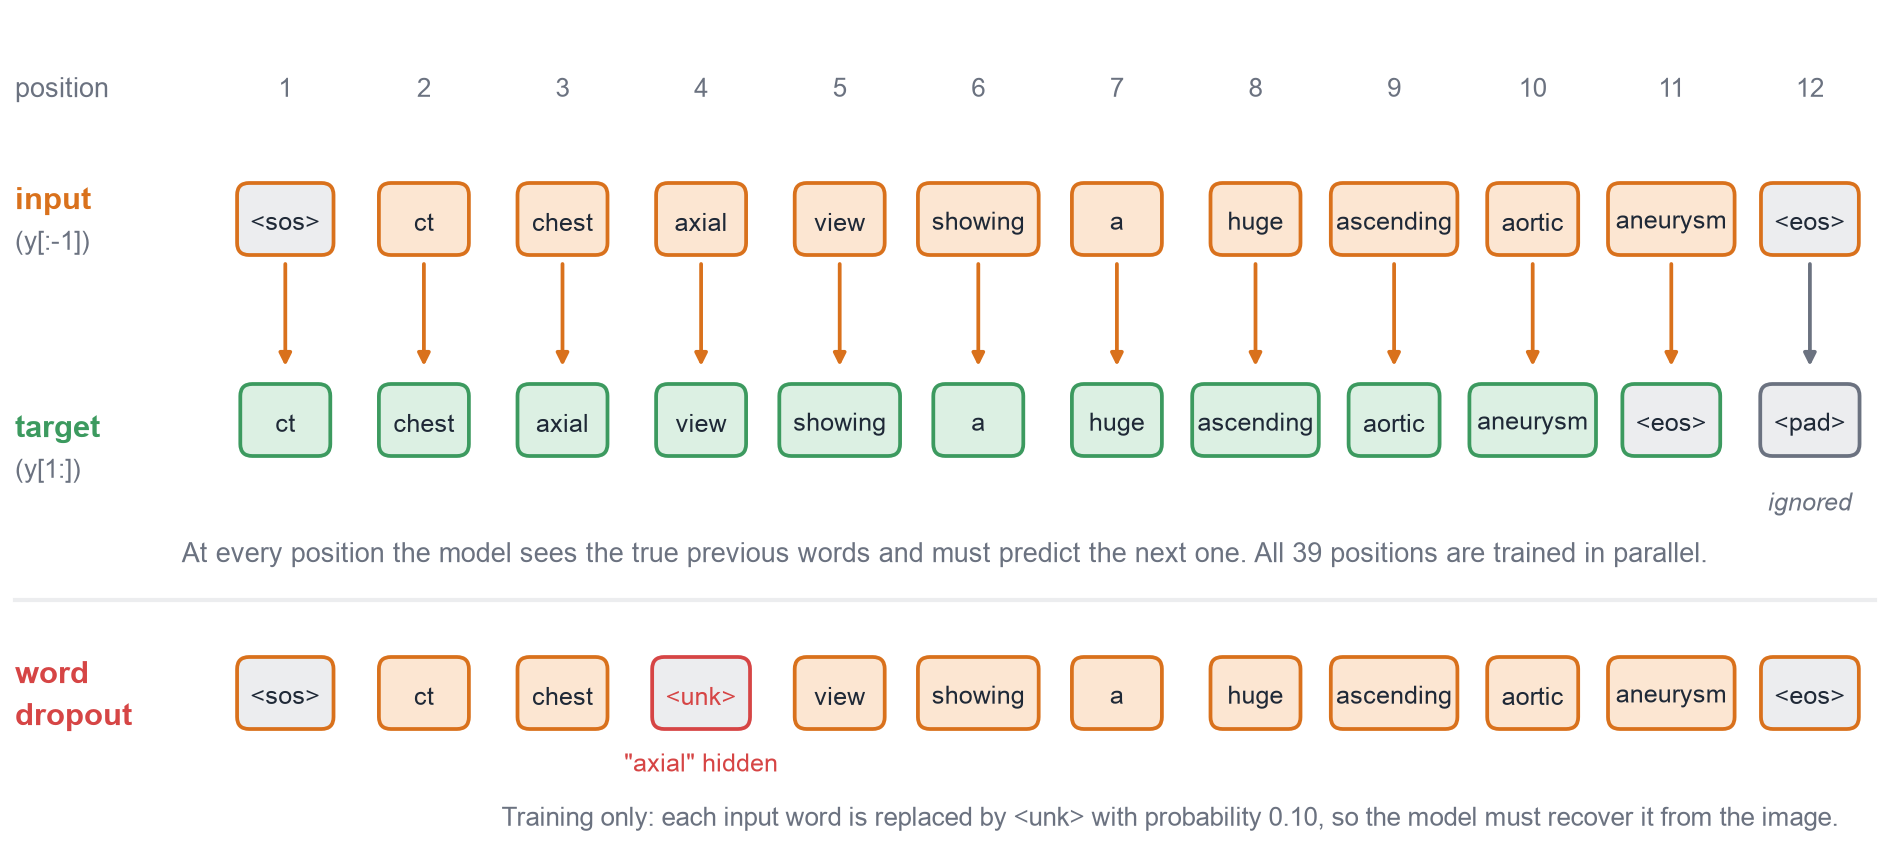
\includegraphics[width=0.92\linewidth,height=\textheight,keepaspectratio]{figures/fig3_21_teacher.png}
\caption{Teacher forcing and word dropout during training. At every position $t$, the decoder processes the ground-truth prefix up to $t-1$ to predict token $y_t$. Word dropout randomly masks input words with $\langle\mathrm{unk}\rangle$ to enforce visual conditioning.}
\end{figure}

\section{Step 7 --- 6-Layer Transformer Decoder Architecture}

The language decoder comprises a stack of $N_{\text{dec}} = 6$ identical Transformer decoder layers. Each layer consists of three residual sub-layers with Layer Normalization:

\begin{figure}[!htbp]
\centering
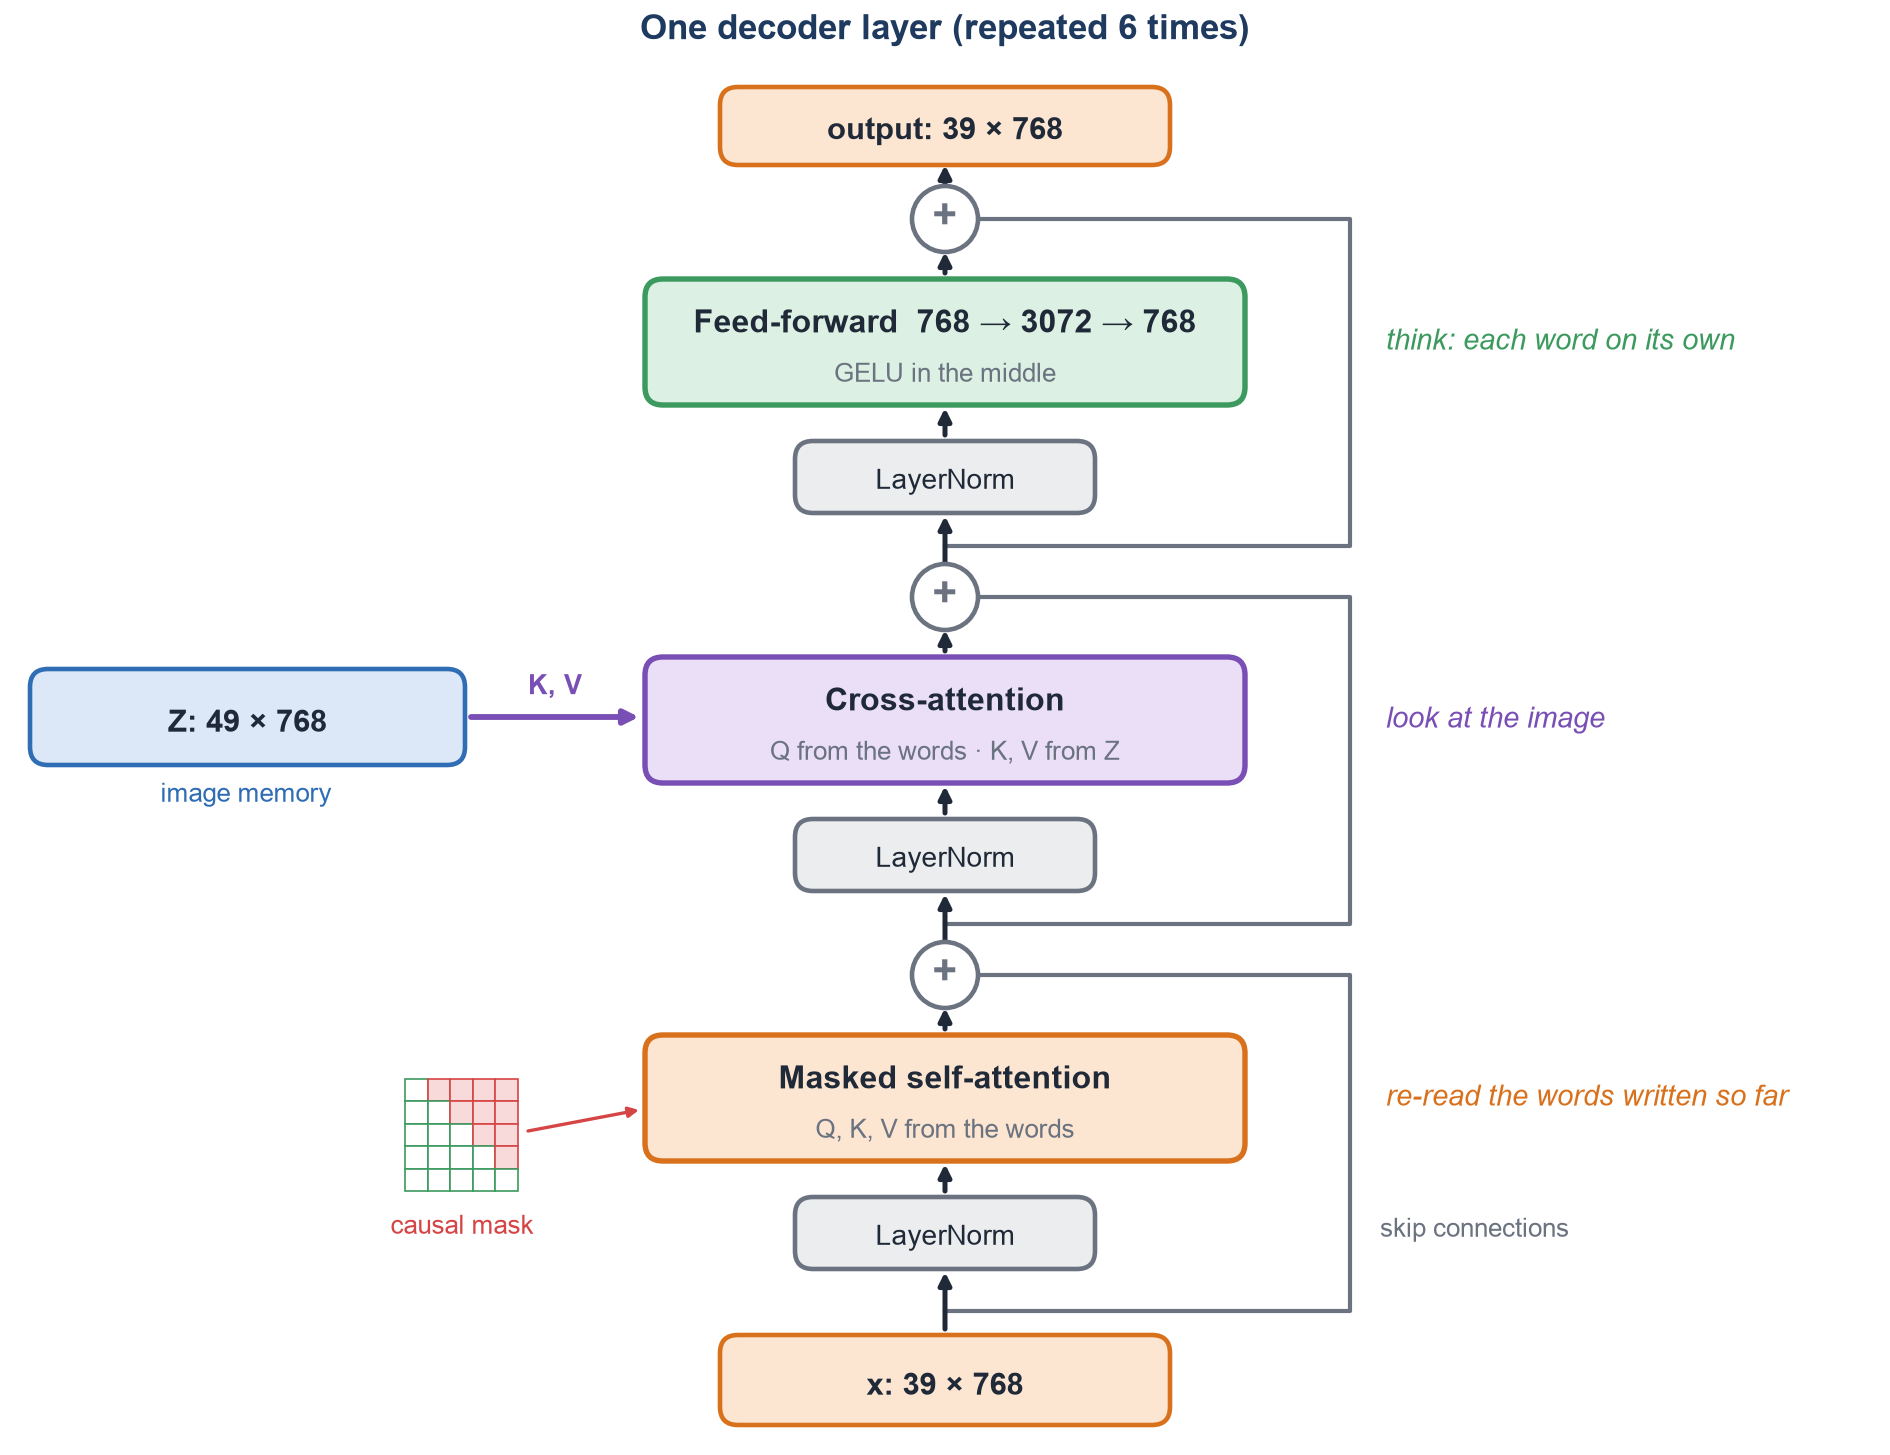
\includegraphics[width=0.75\linewidth,height=\textheight,keepaspectratio]{figures/fig3_22_decoder_layer.png}
\caption{Detailed architectural layout of one Transformer decoder layer. Each layer incorporates causal masked self-attention, visual memory cross-attention, and a position-wise feed-forward network.}
\end{figure}

For layer input $x \in \mathbb{R}^{B \times T' \times 768}$ ($T' = 39$):

\begin{equation}
a = x + \mathrm{Dropout}\left(\text{MHA}_{\text{self}}\left(\mathrm{LN}_1(x);\ \Gamma\right)\right) \tag{3.18}
\end{equation}
\begin{equation}
b = a + \mathrm{Dropout}\left(\text{MHA}_{\text{cross}}\left(\mathrm{LN}_2(a),\ Z\right)\right) \tag{3.19}
\end{equation}
\begin{equation}
x' = b + \mathrm{Dropout}\left(\mathrm{FFN}\left(\mathrm{LN}_3(b)\right)\right) \tag{3.20}
\end{equation}

\subsection{Causal Masked Multi-Head Self-Attention}

Self-attention computes token-to-token contextual dependencies across the generated caption prefix. To enforce autoregressive causality during parallel training, a lower-triangular causal attention mask $\Gamma \in \mathbb{R}^{T' \times T'}$ is applied:

\begin{equation}
\Gamma_{ij} = \begin{cases} 0, & j \le i \quad (\text{past and current tokens: permitted}) \\ -\infty, & j > i \quad (\text{future tokens: masked}) \end{cases} \tag{3.21}
\end{equation}

\begin{equation}
\text{MHA}_{\text{self}}(Q, K, V) = \mathrm{softmax}\left(\frac{Q K^\top}{\sqrt{d_k}} + \Gamma\right) V
\end{equation}

This prevents information leakage from subsequent target tokens during matrix multiplication.

\begin{figure}[!htbp]
\centering
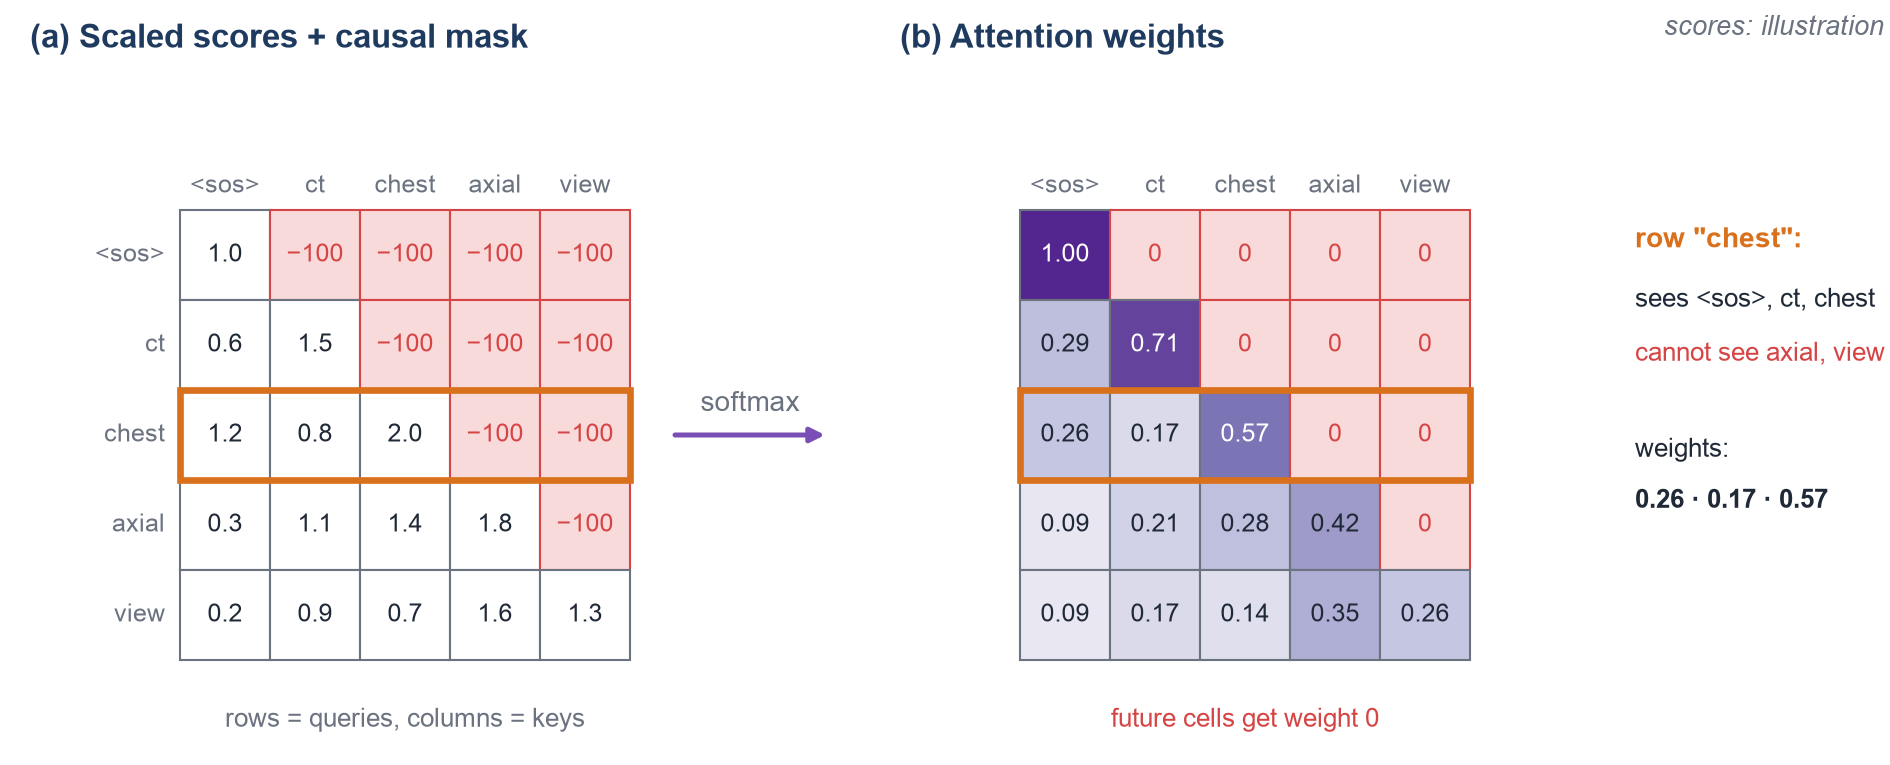
\includegraphics[width=0.88\linewidth,height=\textheight,keepaspectratio]{figures/fig3_29_masked.png}
\caption{Causal self-attention masking. Upper-triangular positions (red) are penalized with $-\infty$, preventing token positions from attending to future sequence targets.}
\end{figure}

\subsection{Visual Memory Cross-Attention}

Cross-attention establishes the core multimodal fusion bridge between visual anatomy and linguistic semantics. The queries ($Q$) are projected from the intermediate decoder state $a$, while keys ($K$) and values ($V$) are projected from the Swin encoder's spatial memory tensor $Z \in \mathbb{R}^{B \times 49 \times 768}$:

\begin{equation}
Q = \mathrm{LN}_2(a) W_Q, \qquad K = Z W_K, \qquad V = Z W_V \tag{3.22}
\end{equation}

where $W_Q, W_K, W_V \in \mathbb{R}^{768 \times 768}$ across 8 parallel attention heads ($d_k = 96$). Because the visual memory retains 49 separate spatial tokens, cross-attention enables each generated word to attend to specific diagnostic regions (e.g., attending to thoracic apex tokens when emitting \emph{``pneumothorax''}).

\begin{figure}[!htbp]
\centering
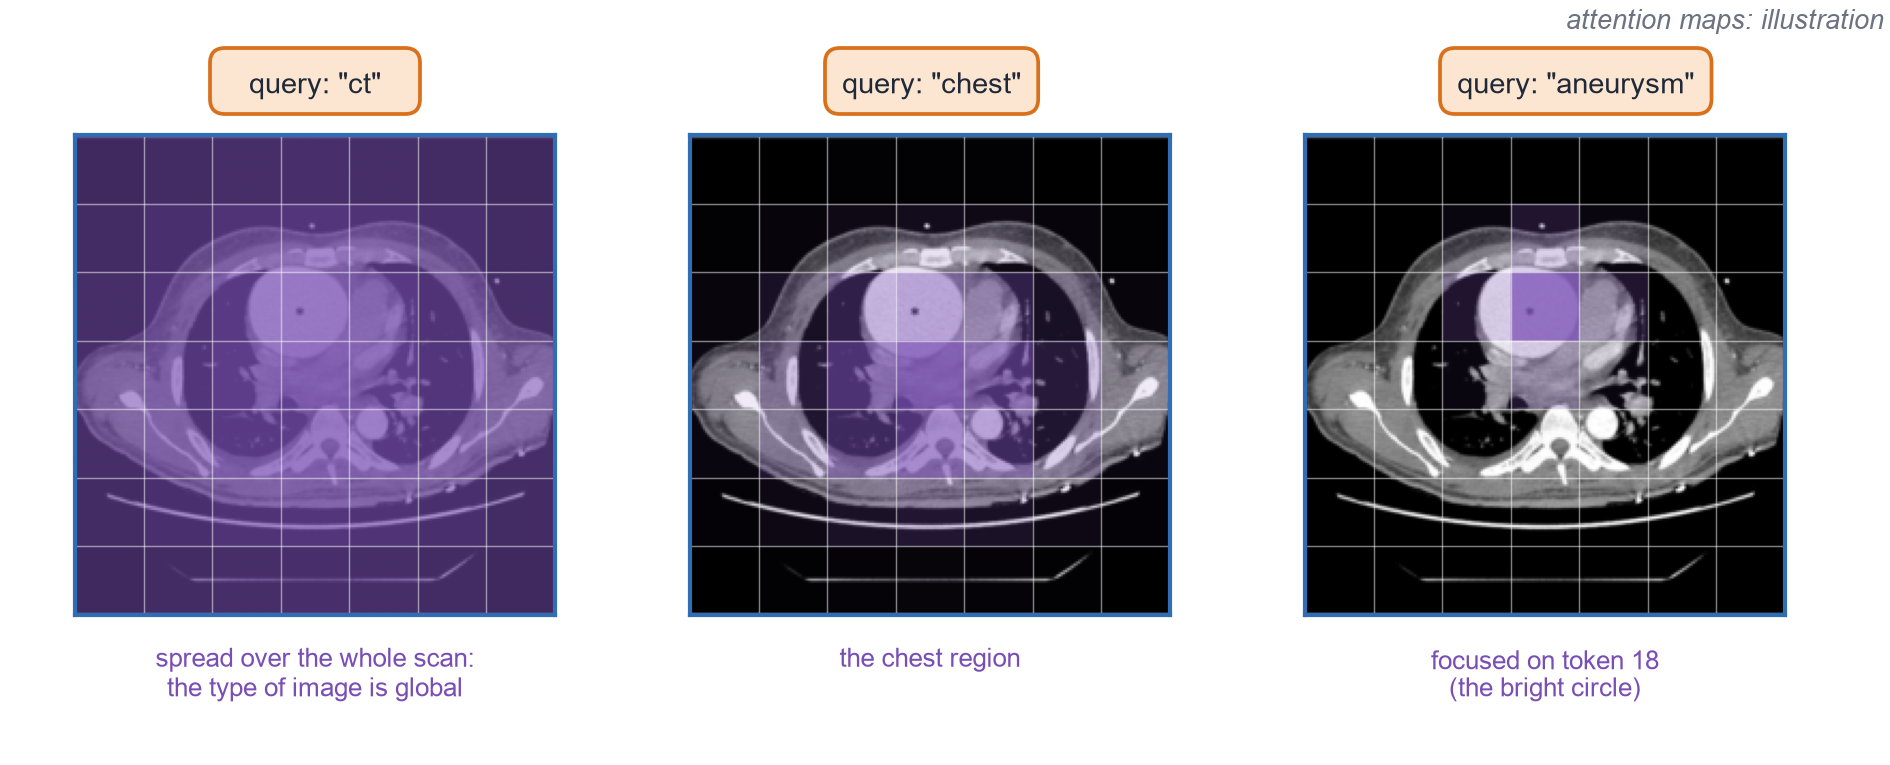
\includegraphics[width=0.92\linewidth,height=\textheight,keepaspectratio]{figures/fig3_30_cross.png}
\caption{Multi-head cross-attention mechanism. Decoder query tokens selectively query the 49 visual memory tokens to ground generated medical findings in specific anatomical regions.}
\end{figure}

\section{Step 8 --- Autoregressive Decoding and Search Strategies}

At inference, ground-truth targets are unavailable. Predictions are generated sequentially:

\begin{figure}[!htbp]
\centering
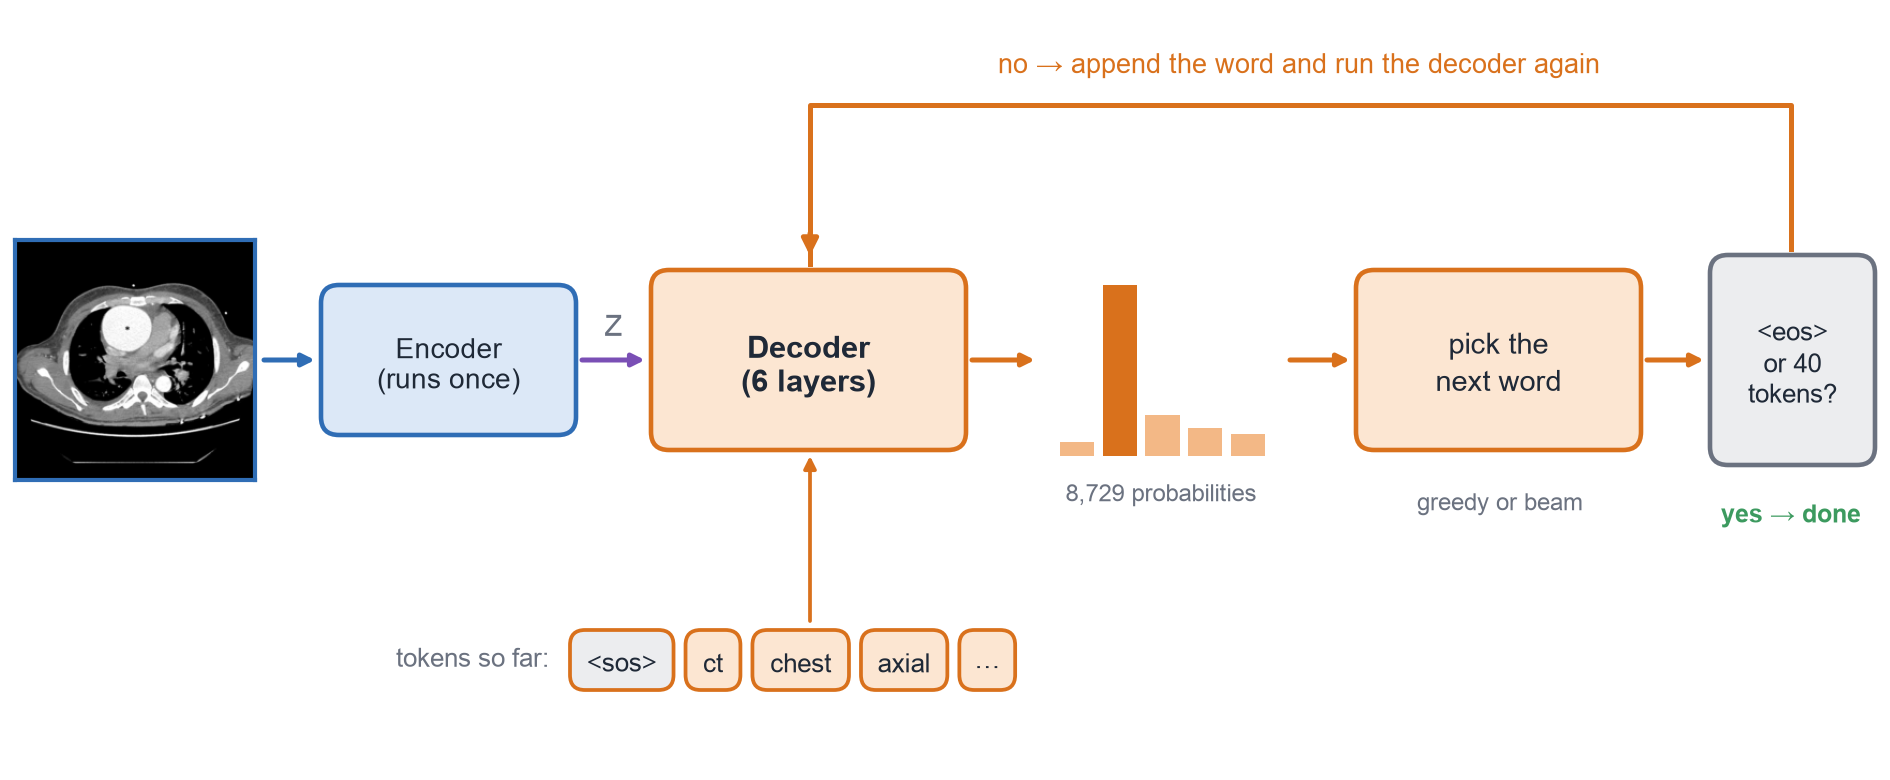
\includegraphics[width=0.85\linewidth,height=\textheight,keepaspectratio]{figures/fig3_31_loop.png}
\caption{Autoregressive decoding loop. At each time step, the candidate token sequence is re-encoded, and the final logit distribution predicts the next vocabulary token until $\langle\mathrm{eos}\rangle$ is emitted.}
\end{figure}

\textbf{1. Greedy Decoding with Repetition Penalties.}
Greedy search selects the token with the highest predicted probability at each step:
\begin{equation}
\hat{y}_{t+1} = \arg\max_{w \in A_t} \ell_t(w)
\end{equation}
To suppress degeneracies, we incorporate immediate previous-token repetition penalties (penalizing $\ell_t(\hat{y}_t)$ by $-100.0$) and trigram blocking (forbidding tri-token loops $(\hat{y}_{t-1}, \hat{y}_t, w)$ seen previously in the sequence).

\textbf{2. Beam Search Decoding ($k=3, 4$).}
While greedy decoding is computationally fast, it cannot recover from early suboptimal selections. We implement length-normalized Beam Search with width $k$:

\begin{equation}
\text{Score}(y_{1:t}) = \frac{\sum_{i=1}^t \log p(y_i | y_{<i}, Z)}{\left(\frac{5 + t}{6}\right)^\alpha}
\end{equation}

where $\alpha = 0.7$ is the length penalty coefficient. At each step, $k$ candidate hypotheses are maintained, filtered through trigram repetition blocking, and ranked to produce fluent, clinically accurate diagnostic text.

\begin{figure}[!htbp]
\centering
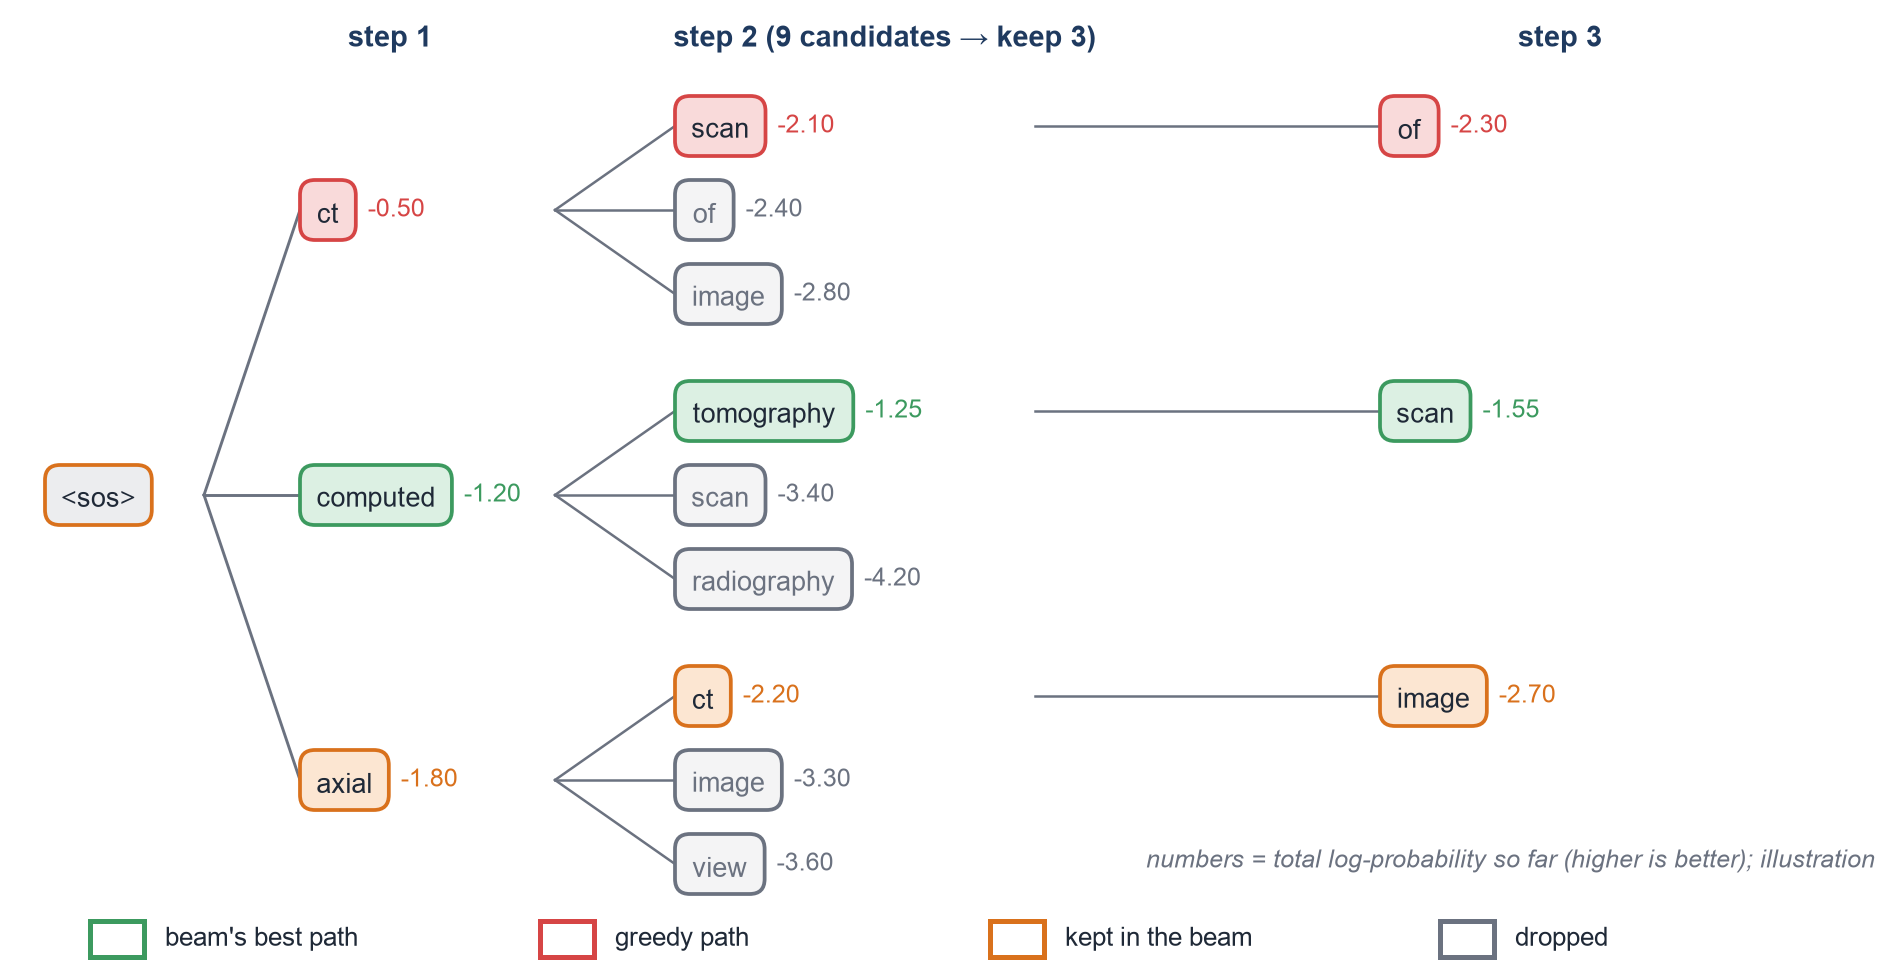
\includegraphics[width=0.88\linewidth,height=\textheight,keepaspectratio]{figures/fig3_32_beam.png}
\caption{Beam search hypothesis tree ($k=3$). Length normalization avoids over-penalizing longer, medically detailed descriptive sentences.}
\end{figure}
